\documentclass{standalone}
\usepackage{tikz,xcolor-material}
\begin{document}
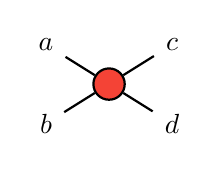
\begin{tikzpicture}[inner sep=4pt, thick, baseline=-0.1cm]
  \path node (M)  at (0,0) [circle, draw, fill=MaterialRed] {}
        node (Ma) at (-0.8, 0.5) {$a$}
        node (Mb) at (-0.8,-0.5) {$b$}
        node (Mc) at ( 0.8, 0.5) {$c$}
        node (Md) at ( 0.8,-0.5) {$d$};
  \draw (M) -- (Ma) (M) -- (Mb) (M) -- (Mc) (M) -- (Md);
\end{tikzpicture}
$\to$
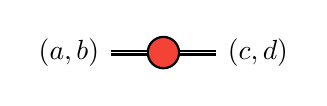
\begin{tikzpicture}[inner sep=4pt, thick, baseline=-0.1cm]
  \path node (M)  at (0,0) [circle, draw, fill=MaterialRed] {}
        node (Mab) at (-1.2,0) {$(a,b)$}
        node (Mcd) at ( 1.2,0) {$(c,d)$};
  \draw [double] (M) -- (Mab) (M) -- (Mcd);
\end{tikzpicture}
\end{document}
